\documentclass[a4paper,10pt]{article}
\usepackage[utf8]{inputenc}

\title{Notes about theory of merge}
\author{Guillaume Bertholon}

\usepackage{listings-rust}
\lstset{
  language=Rust,
  breaklines=true,
  extendedchars=true,
  captionpos=b,
  style=boxed
}

\usepackage{tikz}
\usetikzlibrary{calc}
\usetikzlibrary{positioning}
\usetikzlibrary{shapes.geometric}
\tikzstyle{varnode} = [draw, circle, text height=1.5ex, text depth=.25ex, align=center]
\tikzstyle{modnode} = [draw, rectangle]
\tikzstyle{condnode} = [draw, diamond]
\tikzstyle{conflict} = [red, fill=red!10]
\tikzstyle{colorA} = [fill=blue!30]
\tikzstyle{colorB} = [fill=orange!40]
\tikzstyle{colorC} = [fill=olive!30]
\tikzstyle{colorD} = [fill=teal!30]

\usepackage{bussproofs}
\usepackage{amsmath}
\newcommand{\typsep}{\ |\ }

\usepackage{hyperref}
\hypersetup{hidelinks}

\usepackage[section]{placeins}

\begin{document}

\maketitle

How can we compose simulataneous changes?

\section{Definitions}

\paragraph{Commits \& modifications}
In this section, I will have a very generic notion of commits. A commit is a set of modifications of the semantic of a program. A single modification
can have an impact on several program states and several program variables.
An example of a modification is the change of an expression in an assignment (\lstinline{x = expr}). This modification does not only touch the program variable \lstinline{x} but also each expression that depend the new value in the rest of the program.
\begin{lstlisting}[caption=Modification of $x$]
let mut x = 0; // changed
let y = x + 1; // touched (x is changed)
let z = y + 1; // touched (y is touched)
x = 45;        // untouched
let w = x - 3; // untouched (x have been reassigned)
\end{lstlisting}
Inside a commit we consider that all the modifications are compatible with each
other as their author have thought of their potential interactions.
With this idea of thoughtful interactions, we can consider that sequential commits can always be (virtually) squashed into a single commit before merging.

\paragraph{Concurrent commits}
Concurrent commits are commits that all transform the same initial program. Their authors were not aware of the modifications contained in other commits. Nonetheless, we want to be able to merge the modifications contained in all of them inside a single commit from the common source. A merged version is not always uniquely well-defined because concurrent modifications can (and will often) touch the same program states or variables and therefore collide. That's why there can be several merged versions of the same set of concurrent commits.

Sometimes however they will never collide and a canonical merge commit will naturally exist. This is the case for instance if two incompatible branches are modified by concurrent commits.
\begin{lstlisting}[caption=Merged version of two compatible concurrent commits modifying $x$]
let x;
if (c) {
    x = 1; // changed in first concurrent commit
} else {
    x = 2; // changed in second concurrent commit
}
let y = x + 1; // touched but unambiguous
\end{lstlisting}

\section{Syntactic merge}
If we want to merge concurrent commits into a single one, we need to be able to define a good merged commit. This should yield an executable merged program with provenance annotations that enable to retrieve the origin of a given expression.

Standard tools (like diff or git) are using a line based merge. But in most languages, a line do not have any defined semantic. Therefore, I have taken the approach that concurrent commits should be merged in a syntax driven way.

The high level approach to this syntactic merge is to first compute individual differences from the common ancestor to each commit, and then merge the differences trees into a singe one. Finally, we can apply the merged difference tree to the common ancestor and obtain a syntactically valid merge candidate (but maybe not semantically interesting, and not even necessarily free from compile-time errors).

\subsection{Syntax tree difference}
We want a rather rich way of describing differences to prevent as much as possible useless syntactic conflicts.
Therefore our syntax tree difference structure will encode local tree modification, list insertion and deletion and a notion of typed multi-source, multi-target code move.

\subsubsection{Type for syntax tree differences}
We encode program differences as a new kind of syntax tree that follows the constructors from the target language and add new ones.

Basically, a difference can be viewed as two syntax trees, a deleted one, and an inserted one. Therefore the simplest valid difference from code $d$ to code $i$ is simply the pair $(d, i)$.

However, to ease fusion, produce better output and remove redundancy we change two things.
First, we ellide identical subtrees that are present in both $d$ and $i$.
Secondly, we merge together identical constructions between the deletion and insertion tree starting from the root.

The ellisions can be seen as code moved from a location in $d$ into another location in $i$, but the actual content is temporarily forgotten inside what we call a metavariable. In this paper, we will denote these ellisions by $\alpha, \beta, \gamma,$ and so on.

Trying to merge together two nodes in the AST is easy, we simply need to check if they use the same root constructor, recursively merge if it is the case, and fail otherwise. However, this approach is really bad with sequences (eg. sequences of functions or sequences of statements). We do not want to fully split a list if only one element has been inserted, removed or changed. Therefore, we use list edit scripts instead as the output of a merge operation on two sequences. We call the merged part of the difference tree its spine.

We denote by $S(\overrightarrow{t}, \overrightarrow{s})$ a constructor from the target language AST, with an arbitrary but fixed arity of trees ($t$) and sequences ($s$).

This gives the following types for difference trees:
\begin{align*}
c &::= S(\overrightarrow{c}, \overrightarrow{c}) \typsep \alpha\\
t &::= S(\overrightarrow{t}, \overrightarrow{s}) \typsep id \typsep (c, c)\\
s &::= Zip(t) \typsep Del(c) \typsep Ins(c)\\
\end{align*}

\subsubsection{Computing a syntactic difference}
To compute a syntactic difference, we take ASTs of both the original and the modified program and we run the following algorithm:
\begin{itemize}
  \item Compute a hash for each node of each AST.
  \item Take the subset of hashes occuring both in original and modified AST.
  \item Ellide the nodes with a hash in the subset to remember just their hash.
  \item If an ellided node do not match an ellision with the same hash in the other tree, replace it by the original subtree.
  \item Merge both AST into a common spine where possible, else keep changes as two separate ellided trees. Always try to align sequences using recursively a dynamic algorithm minimizing the number of nodes of the resulting tree.
  \item Optionally, replace each hash by a metavariable index for readability and simplicity.
\end{itemize}

This algorithm is in $O(n*m)$ where $n$ (resp. $m$) is the number of node of the original (resp. modified) tree. The most computationally expansive part of the algorithm is computing sequence alignments, all the rest is linear.

\subsection{Merging differences}
Now that we have difference trees for each individual concurrent change, we can try to merge them in a way that keeps track of the origin of each piece of code.

However, as with line based merge, this merging operation can and will regularly fail if someone wants to merge syntactically incompatible changes.

We therefore break the symmetry between deletion and insertion trees as there will be only one deletion and multiple insertions, and we need to extend our difference types to accumulate potential conflicts.

\begin{align*}
d &::= S(\overrightarrow{d}, \overrightarrow{d}) \typsep \alpha \typsep MvConflict(\alpha, d, i) \\
i &::= S(\overrightarrow{i}, \overrightarrow{j}) \typsep \alpha \typsep Conflict(\overrightarrow{i})\\
j &::= Node(i) \typsep DelConflict(i) \typsep OrdConflict(\overrightarrow{i})\\
t &::= S(\overrightarrow{t}, \overrightarrow{s}) \typsep id \typsep (d, i)\\
s &::= Zip(t) \typsep Del(d) \typsep DelConflict(d, i) \typsep Ins(i) \typsep OrdConflict(\overrightarrow{\overrightarrow{i}})\\
\end{align*}

\subsection{Specification of the difference merging algorithm}
The difference merging algorithm is defined modulo two replacement functions $\Gamma$ and $\Delta$ from metavariable to respectively insertion and deletion trees, that are heavily constrained and in practice inferred during the merge.

\begin{prooftree}
 \AxiomC{$\Gamma, \Delta \vdash t_r \circ t_l = t$}
 \UnaryInfC{$\Gamma, \Delta \vdash t_l \circ t_r = t$}
\end{prooftree}

\subsubsection{Merge spine nodes}
\begin{prooftree}
 \AxiomC{}
 \UnaryInfC{$\Gamma, \Delta \vdash t \circ id = \Delta(\Gamma(t))$}
\end{prooftree}

\begin{prooftree}
 \AxiomC{$\overrightarrow{\Gamma, \Delta \vdash t_l \circ t_r = t}$}
 \UnaryInfC{$\Gamma, \Delta \vdash S(\overrightarrow{t_l}) \circ S(\overrightarrow{t_r}) = S(\overrightarrow{t})$}
\end{prooftree}

\begin{prooftree}
 \AxiomC{$\Gamma \vdash i_l \not\subset d_r$}
 \AxiomC{$\Gamma \vdash i_r \not\subset d_l$}
 \AxiomC{$\Gamma \vdash d_l$}
 \AxiomC{$\Gamma \vdash d_r$}
 \QuaternaryInfC{$\Gamma, \Delta \vdash (d_l, i_l) \circ (d_r, i_r) = (d_l \wedge d_r, i_l \vee i_r)$}
\end{prooftree}

\begin{prooftree}
 \AxiomC{$\Gamma \vdash i_l \subset d_r = d'$}
 \AxiomC{$\Gamma \vdash i_r \not\subset d_l$}
 \AxiomC{$\Gamma \vdash d_l$}
 \TrinaryInfC{$\Gamma, \Delta \vdash (d_l, i_l) \circ (d_r, i_r) = (d' \wedge d_l, \Gamma(i_r))$}
\end{prooftree}

\begin{prooftree}
 \AxiomC{$\Gamma \vdash i_l \subset d_r$}
 \AxiomC{$\Gamma \vdash i_r \subset d_l$}
 \AxiomC{$\Gamma \vdash d_l$}
 \AxiomC{$\Gamma \vdash d_r$}
 \QuaternaryInfC{$\Gamma, \Delta \vdash (d_l, i_l) \circ (d_r, i_r) = (d_l \wedge d_r, i_l \vee i_r)$}
\end{prooftree}

\subsubsection{Merge sequence edit scripts (except insertions)}
\begin{prooftree}
 \AxiomC{$\Gamma, \Delta \vdash t_l \circ t_r = t$}
 \AxiomC{$\Gamma, \Delta \vdash r_l \circ r_r = r$}
 \BinaryInfC{$\Gamma, \Delta \vdash (Zip(t_l) :: r_l) \circ (Zip(t_r) :: r_r) = Zip(t) :: r$}
\end{prooftree}

\begin{prooftree}
 \AxiomC{$\Gamma \vdash d_l$}
 \AxiomC{$\Gamma \vdash d_r$}
 \AxiomC{$\Gamma, \Delta \vdash r_l \circ r_r = r$}
 \TrinaryInfC{$\Gamma, \Delta \vdash (Del(d_l) :: r_l) \circ (Del(d_r) :: r_r) = Del(d_l \wedge d_r) :: r$}
\end{prooftree}

\begin{prooftree}
 \AxiomC{$t_r = (d_r, i_r)$}
 \AxiomC{$\Gamma \vdash i_r \subset d_l$}
 \AxiomC{$\Gamma \vdash d_r$}
 \AxiomC{$\Gamma, \Delta \vdash r_l \circ r_r = r$}
 \QuaternaryInfC{$\Gamma, \Delta \vdash (Del(d_l) :: r_l) \circ (Zip(t_r) :: r_r) = Del(d_l \wedge d_r) :: r$}
\end{prooftree}

\begin{prooftree}
 \AxiomC{$t_r = (d_r, i_r)$}
 \AxiomC{$\Gamma \vdash i_r \not\subset d_l$}
 \AxiomC{$\Gamma \vdash d_l$}
 \AxiomC{$\Gamma \vdash d_r$}
 \AxiomC{$\Gamma, \Delta \vdash r_l \circ r_r = r$}
 \QuinaryInfC{$\Gamma, \Delta \vdash (Del(d_l) :: r_l) \circ (Zip(t_r) :: r_r) = DelConflict(d_l \wedge d_r, \Gamma(i_r)) :: r$}
\end{prooftree}

\begin{prooftree}
 \AxiomC{$\Gamma \vdash i_l \not\subset d_r$}
 \AxiomC{$\Gamma \vdash i_r \not\subset d_l$}
 \AxiomC{$\Gamma \vdash d_l$}
 \AxiomC{$\Gamma \vdash d_r$}
 \AxiomC{$\Gamma, \Delta \vdash r_l \circ r_r = r$}
 \QuinaryInfC{$\Gamma, \Delta \vdash (DelConflict(d_l, i_l) :: r_l) \circ (DelConflict(d_r, i_r) :: r_r) = DelConflict(d_l \wedge d_r, i_l \vee i_r) :: r$}
\end{prooftree}

\begin{prooftree}
 \AxiomC{$\Gamma \vdash i_l \subset d_r = d'_r$}
 \AxiomC{$\Gamma \vdash i_r \not\subset d_l$}
 \AxiomC{$\Gamma \vdash d_l$}
 \AxiomC{$\Gamma, \Delta \vdash r_l \circ r_r = r$}
 \QuaternaryInfC{$\Gamma, \Delta \vdash (DelConflict(d_l, i_l) :: r_l) \circ (DelConflict(d_r, i_r) :: r_r) = DelConflict(d_l \wedge d'_r, \Gamma(i_r)) :: r$}
\end{prooftree}

\begin{prooftree}
 \AxiomC{$\Gamma \vdash i_l \subset d_r = d'_r$}
 \AxiomC{$\Gamma \vdash i_r \subset d_l = d'_l$}
 \AxiomC{$\Gamma, \Delta \vdash r_l \circ r_r = r$}
 \TrinaryInfC{$\Gamma, \Delta \vdash (DelConflict(d_l, i_l) :: r_l) \circ (DelConflict(d_r, i_r) :: r_r) = Del(d'_l \wedge d'_r) :: r$}
\end{prooftree}

\begin{prooftree}
 \AxiomC{$t_r = (d_r, i_r)$}
 \AxiomC{$\Gamma, \Delta \vdash (DelConflict(d_l, i_l) :: r_l) \circ (DelConflict(d_r, i_r) :: r_r) = r$}
 \BinaryInfC{$\Gamma, \Delta \vdash (DelConflict(d_l, i_l) :: r_l) \circ (Zip(t_r) :: r_r) = r$}
\end{prooftree}

\begin{prooftree}
 \AxiomC{$\Gamma \vdash i_l \not\subset d_r$}
 \AxiomC{$\Gamma \vdash d_r$}
 \AxiomC{$\Gamma \vdash d_l$}
 \AxiomC{$\Gamma, \Delta \vdash r_l \circ r_r = r$}
 \QuaternaryInfC{$\Gamma, \Delta \vdash (DelConflict(d_l, i_l) :: r_l) \circ (Del(d_r) :: r_r) = DelConflict(d_l \wedge d_r, \Gamma(i_l)) :: r$}
\end{prooftree}

\begin{prooftree}
 \AxiomC{$\Gamma \vdash i_l \subset d_r = d'_r$}
 \AxiomC{$\Gamma \vdash d_l$}
 \AxiomC{$\Gamma, \Delta \vdash r_l \circ r_r = r$}
 \TrinaryInfC{$\Gamma, \Delta \vdash (DelConflict(d_l, i_l) :: r_l) \circ (Del(d_r) :: r_r) = Del(d_l \wedge d'_r) :: r$}
\end{prooftree}

\subsubsection{Merge insertions in sequence edit scripts}

\begin{prooftree}
 \AxiomC{$s_r \neq Ins(\_)$}
 \AxiomC{$s_r \neq OrdConflict(\_)$}
 \AxiomC{$\Gamma, \Delta \vdash r_l \circ (s_r :: r_r) = r$}
 \TrinaryInfC{$\Gamma, \Delta \vdash (Ins(i_l) :: r_l) \circ (s_r :: r_r) = Ins(\Gamma(i_l)) :: r$}
\end{prooftree}

\begin{prooftree}
 \AxiomC{$\Gamma(i_l) = \Gamma(i_r) = i$}
 \AxiomC{$\Gamma, \Delta \vdash r_l \circ r_r = r$}
 \BinaryInfC{$\Gamma, \Delta \vdash (Ins(i_l) :: r_l) \circ (Ins(i_r) :: r_r) = Ins(i) :: r$}
\end{prooftree}

\begin{prooftree}
 \AxiomC{$\Gamma, \Delta \vdash r_l \circ r_r = r$}
 \UnaryInfC{$\Gamma, \Delta \vdash (Ins(i_l) :: r_l) \circ (Ins(i_r) :: r_r) = OrdConflict([\Gamma(i_l), \Gamma(i_r)]) :: r$}
\end{prooftree}

\begin{prooftree}
 \AxiomC{$s_r \neq Ins(\_)$}
 \AxiomC{$s_r \neq OrdConflict(\_)$}
 \AxiomC{$\Gamma, \Delta \vdash r_l \circ (s_r :: r_r) = r$}
 \TrinaryInfC{$\Gamma, \Delta \vdash (OrdConflict(i_l) :: r_l) \circ (s_r :: r_r) = OrdConflict(\Gamma(i_l)) :: r$}
\end{prooftree}

\begin{prooftree}
 \AxiomC{$\Gamma, \Delta \vdash r_l \circ r_r = r$}
 \UnaryInfC{$\Gamma, \Delta \vdash (Ins(i_l) :: r_l) \circ (OrdConflict(i_r) :: r_r) = OrdConflict(\Gamma(i_l) :: \Gamma(i_r)) :: r$}
\end{prooftree}

\begin{prooftree}
 \AxiomC{$\Gamma, \Delta \vdash r_l \circ r_r = r$}
 \UnaryInfC{$\Gamma, \Delta \vdash (OrdConflict(i_l) :: r_l) \circ (OrdConflict(i_r) :: r_r) = OrdConflict(\Gamma(i_l) @ \Gamma(i_r)) :: r$}
\end{prooftree}

\subsubsection{Inclusion of insertion inside a deletion}

\begin{prooftree}
 \AxiomC{$\overrightarrow{\Gamma \vdash i \subset d = d'}$}
 \UnaryInfC{$\Gamma \vdash S(\overrightarrow{i}) \subset S(\overrightarrow{d}) = S(\overrightarrow{d'})$}
\end{prooftree}

\begin{prooftree}
 \AxiomC{$\Gamma(\alpha) = \Gamma(i)$}
 \UnaryInfC{$\Gamma \vdash i \subset \alpha = \alpha$}
\end{prooftree}

\begin{prooftree}
 \AxiomC{$\Gamma(\alpha) = \top$}
 \UnaryInfC{$\Gamma \vdash i \subset \alpha = MvConflict(\alpha, \alpha, i)$}
\end{prooftree}

\begin{prooftree}
 \AxiomC{$\Gamma(\alpha) = \top$}
 \UnaryInfC{$\Gamma \vdash i \subset MvConflict(\alpha, d, i') = MvConflict(\alpha, d, i \vee i')$}
\end{prooftree}

\begin{prooftree}
 \AxiomC{$d \neq \alpha$}
 \AxiomC{$d \neq S(\_)$}
 \BinaryInfC{$\Gamma \vdash S(\_) \not\subset d$}
\end{prooftree}

\begin{prooftree}
 \AxiomC{$d \neq \alpha$}
 \AxiomC{$i \neq S(\_)$}
 \BinaryInfC{$\Gamma \vdash i \not\subset d$}
\end{prooftree}

\subsubsection{Coherence with $\Gamma$ of kept deletion trees}

\begin{prooftree}
 \AxiomC{$\overrightarrow{\Gamma \vdash d}$}
 \UnaryInfC{$\Gamma \vdash S(\overrightarrow{d})$}
\end{prooftree}

\begin{prooftree}
 \AxiomC{$\Gamma(\alpha) \in \{ \oplus(\Delta(\alpha)), \top \}$}
 \UnaryInfC{$\Gamma \vdash \alpha$}
\end{prooftree}

Where $\oplus$ is a function transposing a deletion tree to an insertion tree by passing through each $MvConflict$ constructor so that $\oplus(MvConflict(\alpha, d, i)) = \oplus(d)$.

\begin{prooftree}
 \AxiomC{$\Gamma(\alpha) = \top$}
 \AxiomC{$\Gamma \vdash d$}
 \BinaryInfC{$\Gamma \vdash MvConflict(\alpha, d, i)$}
\end{prooftree}

\subsubsection{Deletion intersection}
\begin{prooftree}
 \AxiomC{$\overrightarrow{\Delta \vdash d_l \wedge d_r = d}$}
 \UnaryInfC{$\Delta \vdash S(\overrightarrow{d_l}) \wedge S(\overrightarrow{d_r}) = S(\overrightarrow{d})$}
\end{prooftree}

\begin{prooftree}
 \AxiomC{}
 \UnaryInfC{$\Delta \vdash \alpha \wedge \alpha = \Delta(\alpha)$}
\end{prooftree}

\begin{prooftree}
 \AxiomC{$\Delta \vdash \Delta(\alpha) \wedge d_r = \Delta(\alpha)$}
 \UnaryInfC{$\Delta \vdash \alpha \wedge d_r = \Delta(\alpha)$}
\end{prooftree}

\begin{prooftree}
 \AxiomC{$\Delta \vdash \Delta(\alpha) \wedge d_l = \Delta(\alpha)$}
 \UnaryInfC{$\Delta \vdash d_l \wedge \alpha = \Delta(\alpha)$}
\end{prooftree}

\begin{prooftree}
 \AxiomC{$\Delta \vdash d_l \wedge d_r = d$}
 \UnaryInfC{$\Delta \vdash d_l \wedge MvConflict(\alpha, d_r, i) = MvConflict(\alpha, d, \Gamma(i))$}
\end{prooftree}

\begin{prooftree}
 \AxiomC{$\Delta \vdash d_l \wedge d_r = d$}
 \UnaryInfC{$\Delta \vdash MvConflict(\alpha, d_l, i) \wedge d_r = MvConflict(\alpha, d, \Gamma(i))$}
\end{prooftree}

\subsubsection{Simplification of insertion union}

\begin{prooftree}
 \AxiomC{$\Gamma(i_l) = \Gamma(i_r) = i$}
 \UnaryInfC{$\Gamma \vdash i_l \vee i_r = i$}
\end{prooftree}

\begin{prooftree}
 \AxiomC{$\overrightarrow{\Gamma \vdash i_l \vee i_r = i}$}
 \UnaryInfC{$\Gamma \vdash S(\overrightarrow{i_l}) \vee S(\overrightarrow{i_r}) = S(\overrightarrow{i})$}
\end{prooftree}

\begin{prooftree}
 \AxiomC{}
 \UnaryInfC{$\Gamma \vdash i_l \vee i_r = Conflict(\Gamma(i_l), \Gamma(i_r))$}
\end{prooftree}

\section{Semantic merge}
\paragraph{TODO} Update this section!

Having two commits syntactically merged do not mean that the result is a valid
semantic combination that respect the intention of all original commits.
That's why after this first syntax step, we must also check the semantic of the
fusion.

\subsection{A key principle: mandatory disambiguation}
\paragraph{A generic definition of a valid merge} A merge is valid if for any state of the program, there is a single unambiguous trace after applying all the modifications of the concurrent commits. There should be no automatic choice in favor of any of the commits. This means that if two commits touched the same state of the program or the same expression at the same time, the merge will be considered not valid. We call a point in a trace where the semantic is ambiguous a collision.
Note that I consider that this includes a case where commit $A$ modifies a variable $x$ and then commit $B$ changes the value of $y$ to the new value of $x$.

\noindent
\begin{minipage}{.32\textwidth}
\begin{lstlisting}
// Commit A
let x = 2;
let y = 3;
\end{lstlisting}
\end{minipage}\hfill
\begin{minipage}{.32\textwidth}
\begin{lstlisting}
// Original
let x = 1;
let y = 3;
\end{lstlisting}
\end{minipage}\hfill
\begin{minipage}{.32\textwidth}
\begin{lstlisting}
// Commit B
let x = 1;
let y = x; // !!!
\end{lstlisting}
\end{minipage}
\vspace{-.4cm}
\begin{lstlisting}[label=lst:change_introducing_modified, caption={Colliding changes by using a variable modified by someone else}]
\end{lstlisting}

\paragraph{Origin graphs for functionnal programs} To keep track of potential collisions we can create a graph of origins that is updated between each program state. In a program where variables are never mutable, this graph has a node for each variable plus one node for each modification (labelled by the commit). Two nodes are linked by an edge if the value of a variable comes from the value of another variable or comes directly from a modification.

If at a given point of a program, a node of the origin graph is transitively linked to modifications of different concurrent commits, then there is a collision on the variable definition.

\begin{figure}[ht]
\centering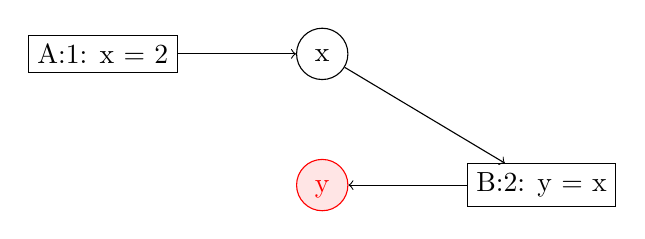
\begin{tikzpicture}
  \node[varnode] (x) {x};
  \node[varnode, below=1cm of x, conflict] (y) {y};

  \node[modnode, left=1.5cm of x] (x_A) {A:1: x = 2};
  \draw[->] (x_A) -- (x);

  \node[modnode, right=1.5cm of y] (y_B) {B:2: y = x};
  \draw[->] (x) -- (y_B);
  \draw[->] (y_B) -- (y);
\end{tikzpicture}
\caption{Illustration of the origin graph of the program showed in listing \ref{lst:change_introducing_modified}. There is a collision for $y$ because it is both linked to a modification in $A$ and a modification in $B$.}
\label{fig:change_introducing_modified}
\end{figure}

\begin{figure}[ht]
\begin{minipage}{.5\textwidth}
\begin{lstlisting}
let a = 0; // Modified by A
let b = 1; // Modified by B
let c = a + b; // Collision
\end{lstlisting}
\end{minipage}\hfill
\begin{minipage}{.45\textwidth}
\centering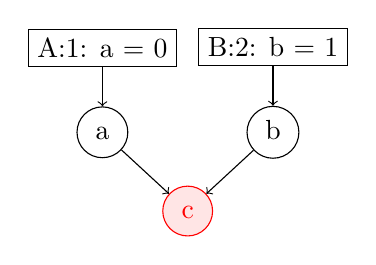
\begin{tikzpicture}
  \node[varnode] (a) {a};
  \node[varnode, right=1.5cm of a] (b) {b};
  \node[varnode, conflict] (c) at ($(a)!0.5!(b)+(0,-1)$) {c};

  \node[modnode, above=0.5cm of a] (A_a) {A:1: a = 0};
  \node[modnode, above=0.5cm of b] (B_b) {B:2: b = 1};

  \draw[->] (A_a) -- (a);
  \draw[->] (B_b) -- (b);
  \draw[->] (a) -- (c);
  \draw[->] (b) -- (c);
\end{tikzpicture}
\end{minipage}
\caption{Collision created after modification of two independant variables}
\end{figure}
\FloatBarrier

\paragraph{Origin graph and control flow} If the value of a variable is used for defining control flow, all the variables inside the branches will gain a dependancy on it.

However incompatible branches can be treated independantly and do not generate conflicts by themselves.

\begin{figure}[ht]
\begin{minipage}{.5\textwidth}
\begin{lstlisting}
let b = 2; // Modified by B
let x =
    if (c) {
        1 // Modified by A
    } else {
        b // Touched by B
    };
let y = x - 1; // OK
let z = y + b; // Conflict
\end{lstlisting}
\end{minipage}\hfill
\begin{minipage}{.45\textwidth}
\centering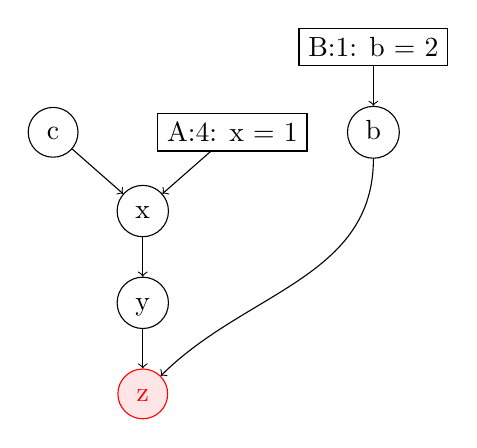
\begin{tikzpicture}
  \node[varnode] (b) {b};
  \node[modnode, above=0.5cm of b] (B_b) {B:1: b = 2};
  \node[modnode, left=0.5cm of b] (A_x) {A:4: x = 1};
  \node[varnode, left=1cm of A_x] (c) {c};
  \node[varnode] (x) at ($(c)!0.5!(A_x)+(0,-1)$) {x};
  \node[varnode, below=0.5cm of x] (y) {y};
  \node[varnode, below=0.5cm of y, conflict] (z) {z};


  \draw[->] (B_b) -- (b);
  \draw[->] (c) -- (x);
  \draw[->] (A_x) -- (x);
  \draw[->] (x) -- (y);
  \draw[->] (y) -- (z);
  \draw[->] (b) to[out=-90, in=45] (z);
\end{tikzpicture}
\end{minipage}
\caption{Origin graph at the end of a program after taking the then branch, showing that there is no collision on $x$ but still one on $z$.}
\label{fig:origin_graph_branches}
\end{figure}

This might become a problem if care is not taken in origin graph checks, because each branch combination might need to be examined.

\paragraph{Solving collisions by overriding}
In order to be able to solve collisions, I extend the definition of a merge with a set of modification overrides in addition to the set of concurrent commits.
A modification in the override set, take precedence over any modification in any of the merged commits. Moreover we can consider that these overrides are done knowing what is inside all the concurrent commits.

In the origin graph, a variable that takes a value defined in by an override modification will loose all incoming arrows as its value is now disambiguated for the current state, taking all further implications into account.

Having a single overriden ancestor can be not enough for marking a conflict as solved though.

\begin{figure}[ht]
\begin{minipage}{.5\textwidth}
\begin{lstlisting}
let a = 0; // modified by A
let b = 1; // modified by B
let o = a + b; // overriden
let c = a + o;
let d = c + b; // Collision!
\end{lstlisting}
\end{minipage}\hfill
\begin{minipage}{.45\textwidth}
\centering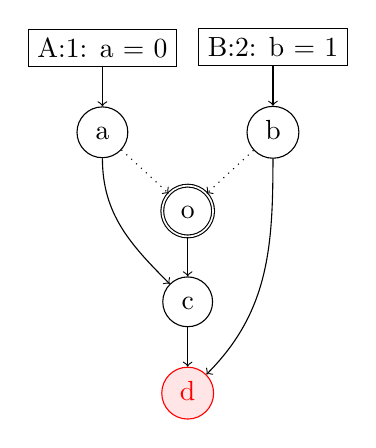
\begin{tikzpicture}
  \node[varnode] (a) {a};
  \node[varnode, right=1.5cm of a] (b) {b};
  \node[varnode, double] (o) at ($(a)!0.5!(b)+(0,-1)$) {o};
  \node[varnode, below=0.5cm of o] (c) {c};
  \node[varnode, below=0.5cm of c, conflict] (d) {d};

  \node[modnode, above=0.5cm of a] (A_a) {A:1: a = 0};
  \node[modnode, above=0.5cm of b] (B_b) {B:2: b = 1};

  \draw[->] (A_a) -- (a);
  \draw[->] (B_b) -- (b);
  \draw[->, dotted] (a) -- (o);
  \draw[->, dotted] (b) -- (o);
  \draw[->] (o) -- (c);
  \draw[->] (c) -- (d);
  \draw[->] (a) to[out=-90,in=135] (c);
  \draw[->] (b) to[out=-90,in=45] (d);
\end{tikzpicture}
\end{minipage}
\caption{Origin graph for a merge with an overriding that solves one conflict line 3 but is insufficient to also solve the conflict line 5. Deleted edges are dotted, variables overriden have a double border.}
\end{figure}

A override can arbitrarily alter a modification, or even touch something that was not modified to restore the intent of both modifications. In the example above, $o$ might have been untouched neither by $A$ or by $B$ or be touch by one of the commits or by both, it doesn't matter. That's why an override is also a way to state the behaviour of the program when the changes are on the same state.

Usually there can be several way to solve the same conflict, but some are more ``powerful'' than others. A variable assigned to an overriden expression should be considered as a variable with a restored semantic with respect to all the modifications.

\begin{figure}[ht]
\begin{minipage}{.5\textwidth}
\begin{lstlisting}
let a = 0; // modified by A
let b = 1; // overriden
let o = a + b;
let c = a + o;
let d = c + b;
\end{lstlisting}
\end{minipage}\hfill
\begin{minipage}{.45\textwidth}
\centering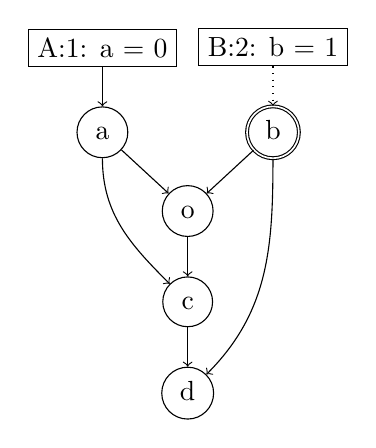
\begin{tikzpicture}
  \node[varnode] (a) {a};
  \node[varnode, right=1.5cm of a, double] (b) {b};
  \node[varnode] (o) at ($(a)!0.5!(b)+(0,-1)$) {o};
  \node[varnode, below=0.5cm of o] (c) {c};
  \node[varnode, below=0.5cm of c] (d) {d};

  \node[modnode, above=0.5cm of a] (A_a) {A:1: a = 0};
  \node[modnode, above=0.5cm of b] (B_b) {B:2: b = 1};

  \draw[->] (A_a) -- (a);
  \draw[->, dotted] (B_b) -- (b);
  \draw[->] (a) -- (o);
  \draw[->] (b) -- (o);
  \draw[->] (o) -- (c);
  \draw[->] (c) -- (d);
  \draw[->] (a) to[out=-90,in=135] (c);
  \draw[->] (b) to[out=-90,in=45] (d);
\end{tikzpicture}
\end{minipage}
\caption{Origin graph for the same example as before except that now line 2 is
overriden marking that $b$ has a preserved semantic. Therefore, line 5 is not showing a conflict anymore.}
\end{figure}

\subsection{From trace to program point origin graphs}
\paragraph{Graph coloring to check conflicts} For being able to quickly check that an assignment does not introduce a conflict, we can simply keep a coloring of the graph, that links each variable to the single unambiguous commit that modifies its semantic.
Therefore a well-formed graph without conflicts only have incoming edges from nodes without coloring or with the same color as itself.
Overriden variables will never be colored as they are considered to never collide with any of the concurrent commits.

\begin{figure}[ht]
\begin{minipage}{.5\textwidth}
\begin{lstlisting}
let b = 2; // Modified by B
let x =
    if (c) {
        1 // Modified by A
    } else {
        b // Touched by B
    };
let y = x - 1; // OK
let z = y + b; // Conflict
\end{lstlisting}
\end{minipage}\hfill
\begin{minipage}{.45\textwidth}
\centering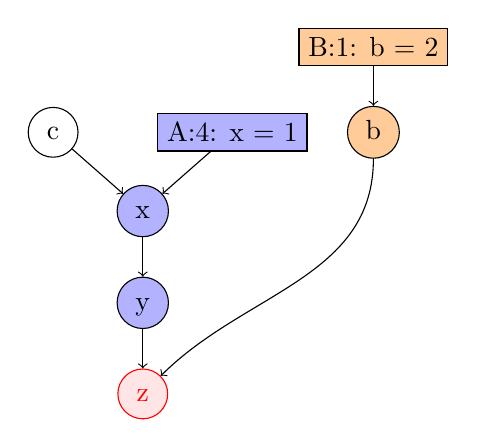
\begin{tikzpicture}
  \node[varnode, colorB] (b) {b};
  \node[modnode, above=0.5cm of b, colorB] (B_b) {B:1: b = 2};
  \node[modnode, left=0.5cm of b, colorA] (A_x) {A:4: x = 1};
  \node[varnode, left=1cm of A_x] (c) {c};
  \node[varnode, colorA] (x) at ($(c)!0.5!(A_x)+(0,-1)$) {x};
  \node[varnode, below=0.5cm of x, colorA] (y) {y};
  \node[varnode, below=0.5cm of y, conflict] (z) {z};


  \draw[->] (B_b) -- (b);
  \draw[->] (c) -- (x);
  \draw[->] (A_x) -- (x);
  \draw[->] (x) -- (y);
  \draw[->] (y) -- (z);
  \draw[->] (b) to[out=-90, in=45] (z);
\end{tikzpicture}
\end{minipage}
\caption{Same origin graph as figure \ref{fig:origin_graph_branches} with coloring}
\label{fig:origin_graph_branches_color}
\end{figure}

\paragraph{Program point origin graph} Also, to ease verification we need to switch from origins graph specified for a given trace to origin graphs specified at a given program point. In absence of control flow expressions, we have no problem for defining it as there is only one trace going from the begining of the program to its end. However we need to deal with conditions and recursive calls (analoguous to loops but in a functional setup) and arbitrary nesting of these two.

A good origin graph at a given program point must be projectable on any trace leading to the program point, and show conflict if at least one of the trace has a conflict.

\paragraph{Conditionals} Join after conditionals seems doable by creating a new color at the join point for each pair of distinct colors in the different branches. New colors should not be created if a variable is not colored in one branch or if it has the same color in both. In these case, it should retain its unambiguous color.

\begin{figure}[!ht]
\centering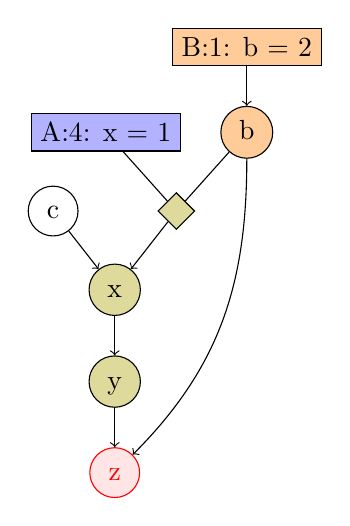
\begin{tikzpicture}
  \node[varnode, colorB] (b) {b};
  \node[modnode, above=0.5cm of b, colorB] (B_b) {B:1: b = 2};
  \node[modnode, left=0.5cm of b, colorA] (A_x) {A:4: x = 1};
  \node[condnode, colorC] (if) at ($(A_x)!0.5!(b)+(0,-1)$) {};
  \node[varnode, left=1cm of if] (c) {c};
  \node[varnode, colorC] (x) at ($(c)!0.5!(if)+(0,-1)$) {x};
  \node[varnode, below=0.5cm of x, colorC] (y) {y};
  \node[varnode, below=0.5cm of y, conflict] (z) {z};

  \draw[->] (B_b) -- (b);
  \draw[->] (c) -- (x);
  \draw (A_x) -- (if);
  \draw (b) -- (if);
  \draw[->] (if) -- (x);
  \draw[->] (x) -- (y);
  \draw[->] (y) -- (z);
  \draw[->] (b) to[out=-90, in=45] (z);
\end{tikzpicture}
\caption{Origin graph for program figure \ref{fig:origin_graph_branches_color} representing all paths going to line 9 at once. Diamonds represent joins after conditional blocks.}
\end{figure}

\begin{figure}[!ht]
\begin{minipage}{.35\textwidth}
\begin{lstlisting}
let x;
if (c) {
    x = 1; // A
} else {
    x = 2; // B
}
let y = x - 1;
let z = x + y;
let u;
if (d) {
    u = 3; // A
} else {
    u = 4; // B
}
let v = z + u; // !
\end{lstlisting}
\end{minipage}\hfill
\begin{minipage}{.6\textwidth}
\centering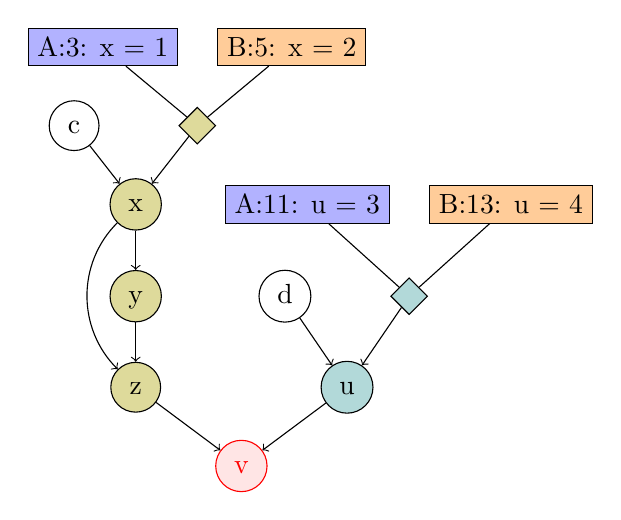
\begin{tikzpicture}
  \node[modnode, colorA] (A_x) {A:3: x = 1};
  \node[modnode, right=0.5cm of A_x, colorB] (B_x) {B:5: x = 2};
  \node[condnode, colorC] (if) at ($(A_x)!0.5!(B_x)+(0,-1)$) {};
  \node[varnode, left=1cm of if] (c) {c};
  \node[varnode, colorC] (x) at ($(c)!0.5!(if)+(0,-1)$) {x};
  \node[varnode, below=0.5cm of x, colorC] (y) {y};
  \node[varnode, below=0.5cm of y, colorC] (z) {z};

  \draw[->] (c) -- (x);
  \draw (A_x) -- (if);
  \draw (B_x) -- (if);
  \draw[->] (if) -- (x);
  \draw[->] (x) -- (y);
  \draw[->] (y) -- (z);
  \draw[->] (x) to[out=-135, in=135] (z);

  \node[modnode, right=0.8cm of x, colorA] (A_u) {A:11: u = 3};
  \node[modnode, right=0.5cm of A_u, colorB] (B_u) {B:13: u = 4};
  \node[condnode, colorD] (ifu) at ({$(A_u)!0.5!(B_u)$} |- y) {};
  \node[varnode, left=1cm of ifu] (d) {d};
  \node[varnode, colorD] (u) at ({$(d)!0.5!(ifu)$} |- z)  {u};
  \node[varnode, conflict] (v) at ($(z)!0.5!(u)+(0,-1)$) {v};

  \draw (A_u) -- (ifu);
  \draw (B_u) -- (ifu);
  \draw[->] (ifu) -- (u);
  \draw[->] (d) -- (u);
  \draw[->] (u) -- (v);
  \draw[->] (z) -- (v);
\end{tikzpicture}
\end{minipage}
\caption{Origin graph at the end of the program summarizing all the possible paths. There is a conflict on $v$ because for example if the green diamond is resolved in favor of $A$ and teal diamond is resolved in favor of $B$, we have an ambiguous value line 15.}
\label{fig:multiple_if}
\end{figure}

We can easily compute the projection on a trace that take a given path by choosing one of the two original colors as a replacement for each color created by merges (and remove the unmatching edges).

An explosion of the number of colors is impossible as the number of colors is bounded at a given point by the number of variables.

This strategy might incur a loss of precision by marking with different colors two distinct conditional expressions on the same condition but is a safe approximation. If necessary, we can refine this by remember the conditions involved to later check that indeed the conflicting case can happen, and print the conflicting path to the user.
\FloatBarrier

\paragraph{Handling recursive functions} In presence of functions we need to add a node for the return value of the function and also add nodes for each functions calls. For the moment, I consider that the result of a function call depends on all the arguments, and only that.

Recursive functions will create some kind of loop in the origin graph (that is representing the implicit looping control flow). Therefore in their presence, we have to be careful and do the coloring after the full construction of the origin graph.
\begin{figure}[!ht]
\begin{minipage}{.5\textwidth}
\begin{lstlisting}
fn f(l: List) -> i32 {
    match l {
        Nil => a,
        Cons(_, t) => b + f(t)
    }
}
\end{lstlisting}
\end{minipage}\hfill
\begin{minipage}{.45\textwidth}
\centering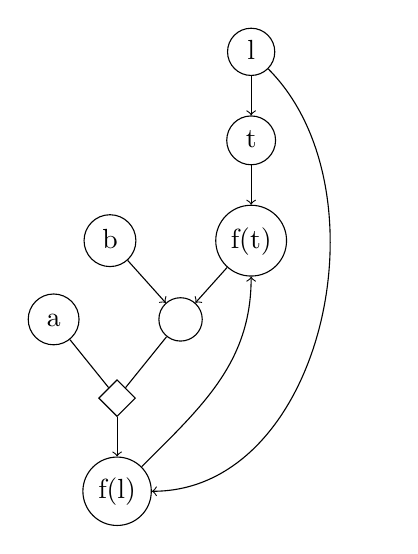
\begin{tikzpicture}
  \node[varnode] (l) {l};
  \node[varnode, below=0.5cm of l] (t) {t};
  \node[varnode, below=0.5cm of t] (ft) {f(t)};
  \node[varnode, left=1cm of ft] (b) {b};
  \node[varnode] (cons_tmp) at ($(ft)!0.5!(b)+(0,-1)$) {};
  \node[varnode, left=1cm of cons_tmp] (a) {a};
  \node[condnode] (switch) at ($(a)!0.5!(cons_tmp)+(0,-1)$) {};
  \node[varnode, below=0.5cm of switch] (res) {f(l)};

  \draw[->] (l) -- (t);
  \draw[->] (t) -- (ft);
  \draw[->] (ft) -- (cons_tmp);
  \draw[->] (b) -- (cons_tmp);
  \draw (a) -- (switch);
  \draw (cons_tmp) -- (switch);
  \draw[->] (switch) -- (res);
  \draw[->] (l) to[out=-45, in=0] (res);
  \draw[->] (res) to[out=45, in=-90] (ft);
\end{tikzpicture}
\end{minipage}
\caption{Origin graph of a recursive function.}
\label{fig:fun_rec}
\end{figure}


\paragraph{Higher order programs with closures} What happens if functions can be inside variables? Seems that simply considering that the function (and all its arguments) is a dependancy of all its calls is enough.

We just need to be careful with captures. A conservative approach would consider that if a function captures a variable, then it gets a dependancy on it. But this can create conflicts that do not exist, if captured variables are used in different branches. A more natural approach is to analyze the inside of the function in the definition environment and then keep the color of the result for the function itself at the end.

\begin{figure}[!ht]
\begin{minipage}{.5\textwidth}
\begin{lstlisting}
let a = 1; // Modified by A
let b = 2; // Modified by B
let f = |x, c| {
    if (c) {
        x + a
    } else {
        x + b
    }
};
let r = f(b, true);
\end{lstlisting}
\end{minipage}\hfill
\begin{minipage}{.45\textwidth}
\centering\begin{tikzpicture}
  \node[varnode, colorA] (a) {a};
  \node[varnode, right=1.5cm of a, colorB] (b) {b};
  \node[modnode, above=0.5cm of b, colorB] (B_b) {B:1: b = 2};
  \node[modnode, above=0.5cm of a, colorA] (A_a) {A:4: x = 1};
  \node[condnode, colorC] (if) at ($(A_x)!0.5!(b)+(0,-1)$) {};
  \node[varnode, below=0.5cm of if, colorC] (f) {f};
  \node[varnode, below=0.5cm of f, conflict] (r) {r};

  \draw[->] (A_a) -- (a);
  \draw[->] (B_b) -- (b);
  \draw (A_x) -- (if);
  \draw (b) -- (if);
  \draw[->] (if) -- (f);
  \draw[->] (f) -- (r);
  \draw[->] (b) to[out=-90, in=45] (r);
\end{tikzpicture}
\end{minipage}
\caption{Origin graph with a closure. The conflict could actually disappear if inlining of $f$ is applied.}
\label{fig:closure}
\end{figure}

\subsection{Oracles for structure preserving modifications}

\paragraph{Modification of expressions only} This idea works very well for commits that only consist of modifications of expressions and preserve the whole program structure (but maybe not the control flow).

If we number all the expressions used in a program, then a commit is a partial map from expression indices to new expressions (and same for the override list).

For conditional branches (\lstinline$if$ or \lstinline$match$), we can consider them both as expressions and as structure. Therefore we can either choose to replace them totally, or to only replace expressions of branches, condition and/or scrutinee.
Obviously, replacing the whole expression, is also a modification of all the branches.

\paragraph{Linking programs before and after commits} For any source program and set of structure preserving modification with matching indices, we can build a correlation oracle that links the program before and the program after the commit together.

The only problem here occurs with programs whose termination status is modified by the commit. To simplify our problem, we will consider first programs that do always terminate.

The correlation oracle can be constructed with as static environment the expression modifications and the origin graph at the end of the program, and as dynamic environment the state of the original program, and the store of the modified program.

The preserved invariant checks that only colored variables in the origin graph have a different value in the store of programs before and after the commit. It should also check the origin of values in the stack.

The interpretation function is executing programs in lockstep manner except that it has to perform a big step if there is a conditional with different conditions in different branches.

If a given program crashes because of a runtime exception, we have to continue executing the other one, relating all its following states to the crashing one.

\paragraph{A correlation oracle to check fusion} Suppose that we have already proven that there is an origin graph including all modifications of all the concurrent commits, with a given list of overrides.

TODO: finish that

\subsection{Checking imperative programs}

\paragraph{Origin graph and mutable variables} In presence of mutable variables we should track not variables but assignment expressions inside the origin graph, and separately keep a link from variables to their definition at the current program point.

\begin{figure}[ht]
\begin{minipage}{.5\textwidth}
\begin{lstlisting}
let a = 2;
let b = 5;
let mut c = a;
while (c < b) {
    c += 1;
}
\end{lstlisting}
\end{minipage}\hfill
\begin{minipage}{.45\textwidth}
\centering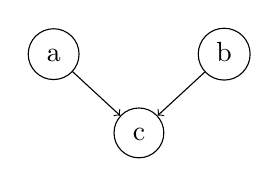
\begin{tikzpicture}
  \node[varnode] (a) {a};
  \node[varnode, right=1.5cm of a] (b) {b};
  \node[varnode] (c) at ($(a)!0.5!(b)+(0,-1)$) {c};

  \draw[->] (a) -- (c);
  \draw[->] (b) -- (c);
\end{tikzpicture}
\end{minipage}
\caption{Origin graph at the end of a program containing a while-loop. Note that $c$ keeps its dependancy on $a$ as it used its previous value inside the loop.}
\end{figure}

\end{document}
